%%%%%%%%%%%%%%%%%%%%%%%%%%%%%%%%%%%%%%%%%
% Beamer Presentation
% LaTeX Template
% Version 1.0 (10/11/12)
%
% This template has been downloaded from:
% http://www.LaTeXTemplates.com
%
% License:
% CC BY-NC-SA 3.0 (http://creativecommons.org/licenses/by-nc-sa/3.0/)
%
%%%%%%%%%%%%%%%%%%%%%%%%%%%%%%%%%%%%%%%%%

%----------------------------------------------------------------------------------------
%	PACKAGES AND THEMES
%----------------------------------------------------------------------------------------

\documentclass{beamer}

\mode<presentation> {

% The Beamer class comes with a number of default slide themes
% which change the colors and layouts of slides. Below this is a list
% of all the themes, uncomment each in turn to see what they look like.

%\usetheme{default}
%\usetheme{AnnArbor}
%\usetheme{Antibes}
%\usetheme{Bergen}
%\usetheme{Berkeley}
%\usetheme{Berlin}
%\usetheme{Boadilla}
%\usetheme{CambridgeUS}
%\usetheme{Copenhagen}
%\usetheme{Darmstadt}
%\usetheme{Dresden}
%\usetheme{Frankfurt}
%\usetheme{Goettingen}
%\usetheme{Hannover}
%\usetheme{Ilmenau}
%\usetheme{JuanLesPins}
%\usetheme{Luebeck}
\usetheme{Madrid}
%\usetheme{Malmoe}
%\usetheme{Marburg}
%\usetheme{Montpellier}
%\usetheme{PaloAlto}
%\usetheme{Pittsburgh}
%\usetheme{Rochester}
%\usetheme{Singapore}
%\usetheme{Szeged}
%\usetheme{Warsaw}

% As well as themes, the Beamer class has a number of color themes
% for any slide theme. Uncomment each of these in turn to see how it
% changes the colors of your current slide theme.

%\usecolortheme{albatross}
%\usecolortheme{beaver}
%\usecolortheme{beetle}
%\usecolortheme{crane}
%\usecolortheme{dolphin}
%\usecolortheme{dove}
%\usecolortheme{fly}
%\usecolortheme{lily}
%\usecolortheme{orchid}
%\usecolortheme{rose}
%\usecolortheme{seagull}
%\usecolortheme{seahorse}
%\usecolortheme{whale}
%\usecolortheme{wolverine}

%\setbeamertemplate{footline} % To remove the footer line in all slides uncomment this line
%\setbeamertemplate{footline}[page number] % To replace the footer line in all slides with a simple slide count uncomment this line

%\setbeamertemplate{navigation symbols}{} % To remove the navigation symbols from the bottom of all slides uncomment this line
}

\usepackage{graphicx} % Allows including images
\usepackage{booktabs} % Allows the use of \toprule, \midrule and \bottomrule in tables
\usepackage{listings}
\usepackage{amsmath}
\usepackage{algpseudocode,algorithm,algorithmicx}

\lstdefinestyle{customjava}{
  breaklines=true,
  frame=L,
  xleftmargin=\parindent,
  language=Java,
  showstringspaces=false,
  basicstyle=\footnotesize\ttfamily,
  keywordstyle=\bfseries\color{green!40!black},
  commentstyle=\itshape\color{gray!40!black},
  identifierstyle=\color{blue},
  stringstyle=\color{orange},
}

\lstdefinestyle{customcpp}{
  breaklines=true,
  frame=L,
  xleftmargin=\parindent,
  language=C++,
  showstringspaces=false,
  basicstyle=\footnotesize\ttfamily,
  keywordstyle=\bfseries\color{green!40!black},
  commentstyle=\itshape\color{gray!40!black},
  identifierstyle=\color{blue},
  stringstyle=\color{orange},
}
%----------------------------------------------------------------------------------------
%	TITLE PAGE
%----------------------------------------------------------------------------------------

\title[Caches]{Caches} % The short title appears at the bottom of every slide, the full title is only on the title page

\author{Jonathan Windle} % Your name
\institute[UEA] % Your institution as it will appear on the bottom of every slide, may be shorthand to save space
{
University of East Anglia \\ % Your institution for the title page
\medskip
\textit{J.Windle@uea.ac.uk} % Your email address
}
\date{\today} % Date, can be changed to a custom date

\begin{document}

\begin{frame}
\titlepage % Print the title page as the first slide
\end{frame}

\begin{frame}[allowframebreaks]
\frametitle{Overview} % Table of contents slide, comment this block out to remove it
\tableofcontents % Throughout your presentation, if you choose to use \section{} and \subsection{} commands, these will automatically be printed on this slide as an overview of your presentation
\end{frame}

%-------------------------------------------------------------------
\section{Principle of locality}
\begin{frame}
\frametitle{Principle of locality}
\begin{itemize}
\item Programs access a small proportion of their address space at any tme.
\item {\color{red}Temporal locality}
\begin{itemize}
\item Items accessed recently are likely to be accesses again soon
\item E.g. Instructions in a loop, induction variables
\end{itemize}
\item {\color{green}Spatial locality}
\begin{itemize}
\item Items near those accessed recently are likely to be accessed soon
\item E.g. Sequential instruction access, array data
\end{itemize}
\end{itemize}
\end{frame}
%-----------------------------------------------------------------------
\section{Basics}
\begin{frame}
\frametitle{Basics}
\begin{itemize}
\item The first time processor reads from an address in the main memory, we can make a copy of the data and put it into the cache memory
\item Next time the data from the same address is needed, we can use its copy that we have stored in the cache
\item The first read was slow, but then every subsequent read is much quicker
\item We have taken advantage of the {\color{red}temporal} locality.
\item We can also take advantage of the {\color{green} spatial} locality
\item Instead of copying only the data from the requested memory address, we can copy the data rsiding nearby e.g. instead of a byte, we can copy the whole word.
\item Next time any of the four bytes are needed, they are available from the cache
\item Of course, the initial loads were slow, but we predict the data will be used soon likely more than once
\end{itemize}
\end{frame}
%---------------------------------------------------------------------
\section{Cache hits and misses}
\begin{frame}
\frametitle{Cache hits and misses}
\begin{itemize}
\item A {\color{red}cache hit} occurs if the data requested by the CPU appears somewhere in the cache
\item If the data is not there, we have a {\color{green}cache miss}
\item Further, we can define a {\color{purple}hit rate} i.e. the fraction of memory accesses found in the cache.
\item Analogously, we define a {\color{orange}miss rate} which is $1-hit rate$.
\item Typically, cache hit rates are above 95\% which tells us that the vast majority of memory accesses are fast since they are handled by the cache.
\end{itemize}
\end{frame}
%------------------------------------------------------------------
\section{A basic cache design}
\begin{frame}
\frametitle{A basic cache design}
\begin{columns}[c]
\column{0.5\textwidth}
\begin{itemize}
\item Each cache consists of {\color{red}blocks}, which take advantage of the spatial locality.
\item Let's assume for a moment that the block size is one byte (no spatial locality yet) 
\item The most basic design is so called {\color{green}direct-mapped} cache where each memory location is mapped to exactly one location in the cache
\end{itemize}
\column{0.5\textwidth}
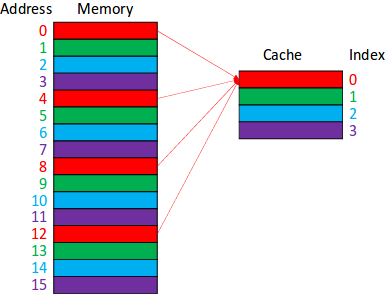
\includegraphics[scale=0.4]{basic.png}
\end{columns}
\end{frame}
%------------------------------------------------------------------
\section{Memory to cache mapping}
\begin{frame}[allowframebreaks]
\frametitle{Memory to cache mapping}
\begin{columns}[c]
\column{0.5\textwidth}
\begin{itemize}
\item The memory address is mapped to the cache index using the mod (remainder) division
\item The size of cache memory is $2^k$
\item Then, the memory address $a$ is mapped to $a\%2^k$
\item E.g. {\color{green} $13\rightarrow13\%4 = 1$}
\end{itemize}
\column{0.5\textwidth}
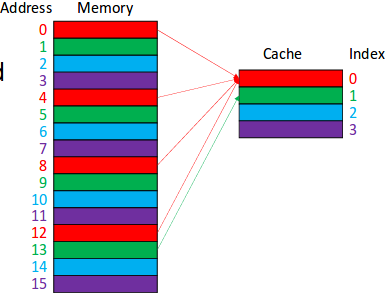
\includegraphics[scale=0.4]{mem.png}
\end{columns}
\framebreak
\begin{columns}[c]
\column{0.5\textwidth}
\begin{itemize}
\item Instead of calculating mod division, could look at k least significant bits of the address
\item E.g. 11{\color{green}01} $\rightarrow$ {\color{green}01}
\end{itemize}
\column{0.5\textwidth}
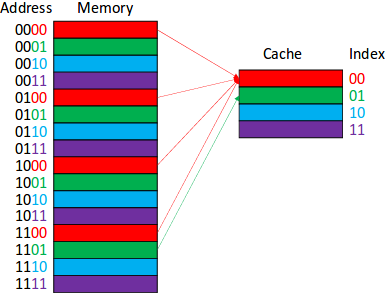
\includegraphics[scale=0.4]{mem2.png}
\end{columns}
\end{frame}
%-----------------------------------------------------------------
\section{Cache tags}
\begin{frame}
\frametitle{Cache tags}
\begin{columns}[c]
\column{0.5\textwidth}
\begin{itemize}
\item Cache blocks need to be supplemented with tags
\item A tag contains the address information necessary to establish whether the associated cache block correspondes to a requested address
\item A tag together with the corresponding index form the corresponding memory address
\item E.g. Tag - {\color{blue} 01} and Index - {\color{red} 00} correspond to memory address: {\color{blue}01}{\color{red}00}.
\end{itemize}
\column{0.5\textwidth}
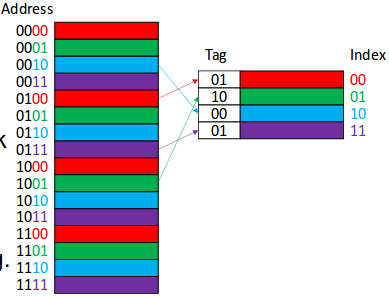
\includegraphics[scale=0.4]{tags.png}
\end{columns}
\end{frame}
%-------------------------------------------------------------------
\section{Valid bit}
\begin{frame}
\frametitle{Valid bit}
\begin{columns}[c]
\column{0.5\textwidth}
\begin{itemize}
\item Initially the cache memory contains invalid daata in all blocks
\item On the first load to the cache block the corresponding {\color{red}valid bit} is set to 1.
\end{itemize}
\column{0.5\textwidth}
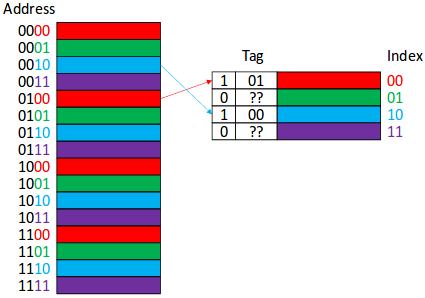
\includegraphics[scale=0.4]{valid.png}
\end{columns}
\end{frame}
%---------------------------------------------------------------------
\section{Cache hit}
\begin{frame}
\frametitle{Cache hit}
\begin{itemize}
\item On memory read, the address is sent to a {\color{red}cache controller}
\item The address is subdivided into lower k bits which index a block and upper bits for tag matching
\item If the block is valid (VB=1) and its tag matches the upper bits of the address, the data is sent to the CPU
\end{itemize}
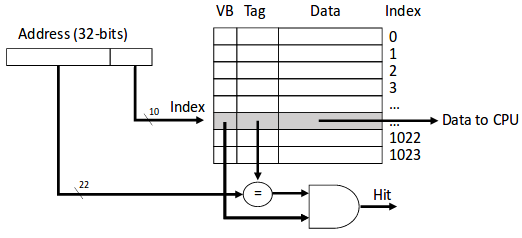
\includegraphics[scale=0.4]{hit.png}
\end{frame}
%---------------------------------------------------------------------
\section{Cache miss}
\begin{frame}
\frametitle{Cache miss}
\begin{itemize}
\item A slow memory access is needed
\item The simplest solution is to stall the pipeline until the data is fetched from memory and copied into cache
\end{itemize}
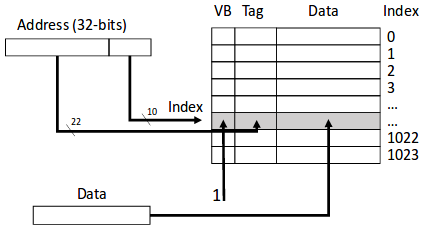
\includegraphics[scale=0.4]{miss.png}
\end{frame}

%-----------------------------------------------------------------------
\section{Cache example}
\begin{frame}
\frametitle{Cache example}
\begin{itemize}
\item 8 blocks, direct-mapped:
\end{itemize}
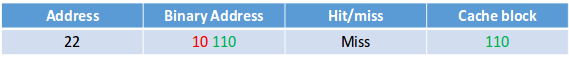
\includegraphics[scale=0.4]{ex1.png}\\
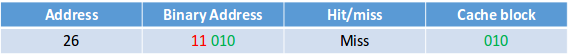
\includegraphics[scale=0.4]{ex2.png}\\
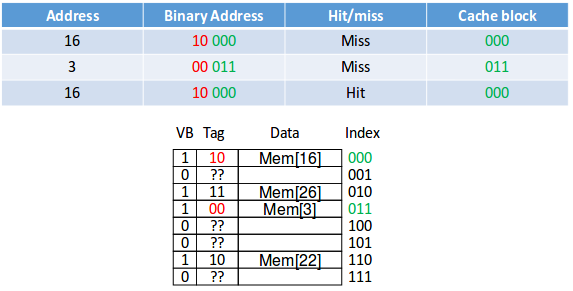
\includegraphics[scale=0.4]{ex3.png}
\end{frame}
%----------------------------------------------------------------------
\section{Cache sizes}
\begin{frame}
\frametitle{Cache sizes}
\begin{itemize}
\item Direct-mapped
\item 1 byte per block
\item 32 blocks
\item handles 16-bit addresses
\end{itemize}
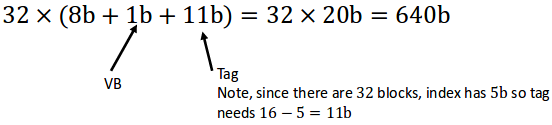
\includegraphics[scale=0.4]{size.png}
\end{frame}
%--------------------------------------------------------------------
\section{Cache performance}
\begin{frame}
\frametitle{Cache performance}
\begin{itemize}
\item {\color{red}Hit time} - Time to access cache, usually 1-3 clock cycles
\item {\color{green}Miss penalty} - Time to move data from memory to cache, at least tens of clock cycles, often a lot longer
\item {\color{orange}Average memory access time (AMAT)}
\begin{itemize}
\item $AMAT=hit \ time + (miss \ rate \times miss \ penalty)$
\item The lower AMAT, the better
\item Since miss penalty is much greater than hit time, the best strategy to lower AMAT is to reduce miss rate or miss penalty
\end{itemize}
\end{itemize}
\end{frame}
\subsection{Example}
\begin{frame}
\frametitle{Example}
\begin{itemize}
\item Say hit rate is 98\%, hit time is one clock cycle and the miss penalty is 50 clock cycles. What is AMAT?
\begin{itemize}
\item $AMAT = 1 + (0.02\times 50) = 2$
\item If hit rate was perfect, the AMAT would be one clock cycle, with a it rate just below 1, the AMA has doubled
\item Spatial locality increases hit rate/reduce miss rate
\end{itemize}
\end{itemize}
\end{frame}
%------------------------------------------------------------------------------
\section{Larger Block Sizes}
\begin{frame}
\frametitle{Larger Block Sizes}
\begin{columns}[c]
\column{0.4\textwidth}
\begin{itemize}
\item Using block size of two:
\item To map memory address to its {\color{red}block address} we use integer division
\item E.g. {\color{green}$10\div2 = 5, 11\div2=5$} 
\item Block address 5 belongs to cache block 1 since $5\%4 = 1$
\end{itemize}
\column{0.6\textwidth}
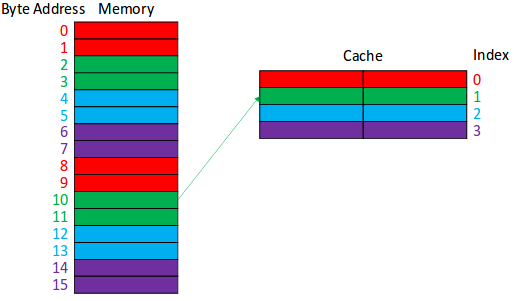
\includegraphics[scale=0.35]{large.png}
\end{columns}
\end{frame}
%-----------------------------------------------------------------
\section{Placement of bytes within a block}
\begin{frame}
\frametitle{Placement of bytes within a block}
\begin{columns}[c]
\column{0.4\textwidth}
\begin{itemize}
\item If a program reads byte 10 from the main memory, we copy both 10 and 11 from the cache
\item The same will happen if the program requests byte 11.
\end{itemize}
\column{0.6\textwidth}
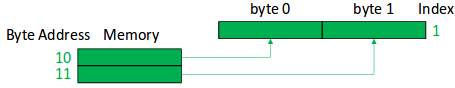
\includegraphics[scale=0.4]{placement.png}
\end{columns}
\end{frame}
%---------------------------------------------------------------------
\section{Building byte address}
\begin{frame}
\frametitle{Building byte address}
\begin{columns}[c]
\column{0.4\textwidth}
\begin{itemize}
\item For $2^k$ cache size and $2^n$ block size:
\item In example:
\begin{itemize}
\item $2^4$ memory size
\item $2^2$ cache size
\item $2^1$ block size
\item Byte 11 (1011)
\end{itemize}
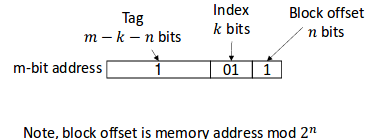
\includegraphics[scale=0.3]{byteex.png}
\end{itemize}
\column{0.6\textwidth}
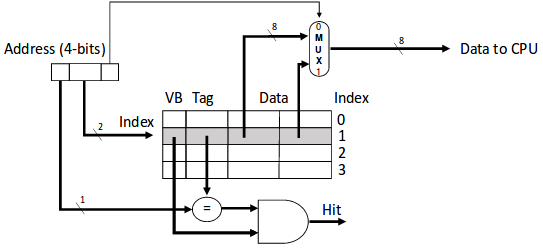
\includegraphics[scale=0.34]{byteex2.png}
\end{columns}
\end{frame}
%-----------------------------------------------------------------
\section{Examples}
\begin{frame}
\frametitle{Examples}
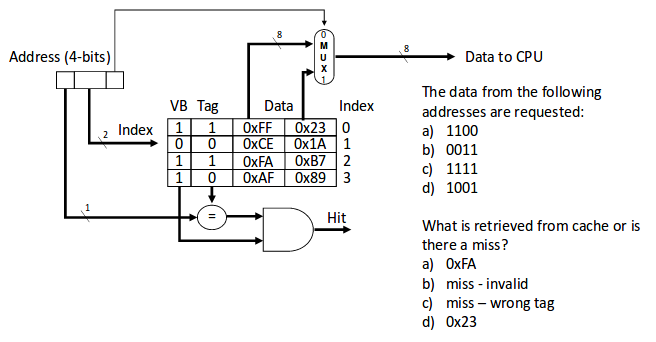
\includegraphics[scale=0.5]{exer.png}
\end{frame}
%-----------------------------------------------------------------
\section{Problem with direct mapping}
\begin{frame}
\frametitle{Problem with direct mapping}
\begin{columns}[c]
\column{0.5\textwidth}
\begin{itemize}
\item Going back to the first example, and the load being 0,4,0,4,0,4 etc
\item Since both map to the same cache block, all loads will be cache misses.
\item The cache contains 4 blocks, and not using them efficiently
\end{itemize}
\column{0.5\textwidth}
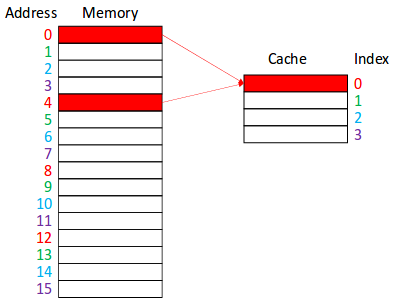
\includegraphics[scale=0.35]{prob.png}
\end{columns}
\end{frame}
%------------------------------------------------------------------
\section{Fully associative cache}
\begin{frame}
\frametitle{Fully associative cache}
\begin{itemize}
\item Unlike direct-mapped cache, a {\color{red}full associative cache} can map a memory address to any block in the cache and hence solves multiple misses issue.
\item If all blocks are full, you could replace the one which was {\color{green}least recently used}
\item The luxury of fully associativecache comes with significantly increased complexity of the hardware
\item No index field and therefore entire address is used as a tag
\item Even worse, the block can be stored anywhere in the cache, so allthe tags have to be compared against required address.
\end{itemize}
\end{frame}
%------------------------------------------------------------------
\section{Set associative cache}
\begin{frame}
\frametitle{Set associative cache}
\begin{itemize}
\item A compromise between the direct mapped cache and the fully associative cache is a {\color{green}set associative cache}.
\item Cache is divided into groups of blocks called sets
\item Each memory address is mapped to only one set. However, the blocks of data can be placed anywhere within this set
\item A {\color{red}$2^x$ -way associative cache} has $2^x$ blocks in each set
\end{itemize}
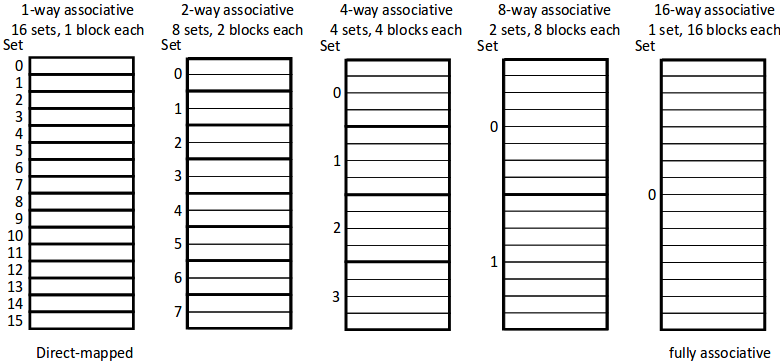
\includegraphics[scale=0.34]{set.png}
\end{frame}
%---------------------------------------------------------------------
\section{Set associative cache addressing}
\begin{frame}
\frametitle{Set associative cache addressing}
\begin{itemize}
\item Similar to direct-mapped.
\item Instead of cache index, use a {\color{red}set index}
\item Assuming a cache has $2^s$ sets and each block $2^n$ bytes, the memory address is subdivided as follows:\\
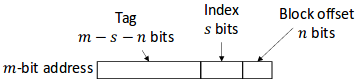
\includegraphics[scale=0.5]{setadd.png}\\
\item The computations of relevant fields are analogous to what was seen earlier.
\end{itemize}
\end{frame}
\subsection{Example}
\begin{frame}
\frametitle{Example}
\begin{itemize}
\item Assuming 16 block design and 16 bytes per block where will the address 7129 be placed:
\begin{itemize}
\item 7129 is 0...011011{\color{red}1101}{\color{blue}1001}:
\item For the 1-way cache, {\color{red}1101}
\item For the 2-way cache, {\color{red}101}
\item For the 4-way cache, {\color{red}01}
\item For the 8-way cache, {\color{red}1}
\end{itemize}
\end{itemize}
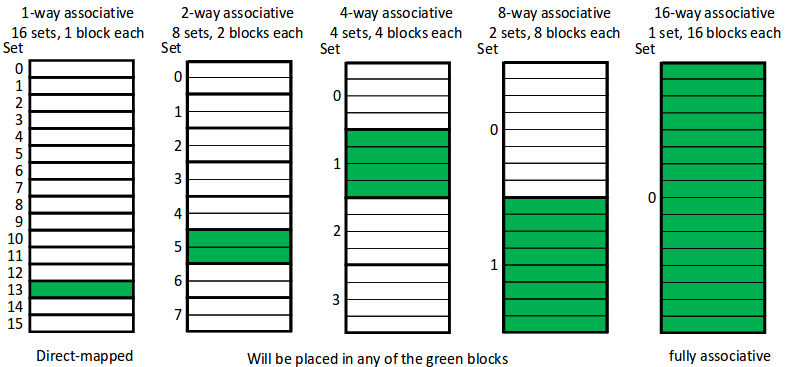
\includegraphics[scale=0.35]{assex.png}
\end{frame}
%--------------------------------------------------------------------
\section{Block replacement strategies}
\begin{frame}
\frametitle{Block replacement strategies}
\begin{itemize}
\item For associative caches, can use any non-empty (invalid) block for new data
\item If all blocks are valid, replace the least recently used block
\item This requires keeping statistics of block access
\item For 2-way associative cache, nly one bit per set, call it LRU, the bit is inverted on every cache miss
\item For highly associative caches, keeping track of the least recently used block may be expensive and often approximations are used.
\end{itemize}
\end{frame}
%------------------------------------------------------------------
\section{Writing to memory}
\begin{frame}
\frametitle{Writing to memory}
\begin{itemize}
\item More complicated that reading
\item Assume the address we want to write is already in the cache, can update its value and avoid slow memory access
\item Now the memory and cache contain inconsistent values
\item This may create problems if the memory is shared with other devices
\end{itemize}
\end{frame}
\subsection{Write-through cache}
\begin{frame}
\frametitle{Write-through cache}
\begin{itemize}
\item A simple solution is  {\color{red}write-through cache} which forces all writes to update both memories
\item But makes writes take longer
\begin{itemize}
\item If base CPI = 1, 10\% of instructions are stores, write to memory takes 100 cycles
\item Effective CPI = $1 + 0.1\times 100 = 11$
\end{itemize}
\item {\color{green} Write buffer} can help with the above problem
\item It will hold data waiting to be written into memory
\item CPU continues immediately
\item Only stalls on write if buffer is already full
\end{itemize}
\end{frame}
\subsection{Write-back cache}
\begin{frame}
\frametitle{Write-back cache}
\begin{itemize}
\item A {\color{red} write-back cache} is an alternate option
\item It updates the memory only if the cache block needs to be replaced
\item We would write the data to cache first and leave it inconsistent with the memory
\item We would mark such a cache block ``dirty" to indicate inconsistency
\item Any subsequent load instruction accessing the same memory would be serviced by the cache
\item The ``dirty" value will be stored in the main memory only after the cache block in which it resides needs to be replaced.
\item The writes can be also buffered as was the case with writ-through cache
\item Write-back cache is potentially more efficient as it takes advantage that not all write operations need to access main memory
\end{itemize}
\end{frame}
%-----------------------------------------------------------------
\section{Write misses}
\begin{frame}
\frametitle{Write misses}
\begin{itemize}
\item Another scenario arises if we want to write to an address that is not contained in the cache - {\color{red}write miss}
\item Two policies:
\begin{itemize}
\item \textbf{Write around:} (write-no-allocate) is advantageous when data is stored, but then is not immediately used again so there is no point of having in the cache yet.
\item \textbf{Write allocate:} is advantageous when data is needed soon
\end{itemize}
\end{itemize}
\end{frame}
%------------------------------------------------------------------
\section{Cache organisations}
\begin{frame}
\frametitle{Cache organisations}
\begin{itemize}
\item Datad/Instruction caches:
\begin{itemize}
\item Pros: No structual hazards between IF and MEM stages
\item Cons: Can be bad if instruction/daata sets are unbalanced
\end{itemize}
\item Cache hierarchies:
\begin{itemize}
\item There is a trade-off between access time and hit rate
\item Smaller L1 cache can focus on access time
\item Larger L2 cache can focus on good hit rate
\end{itemize}
\end{itemize}
\end{frame}
%------------------------------------------------------------------
\section{Larger cache blocks and memory bandwidth}
\begin{frame}[allowframebreaks]
\frametitle{Larger cache blocks and memory bandwidth}
\begin{itemize}
\item Larger cache blocks impose additional miss penalties as we need to perform some number of individual memory acccesses
\item The miss penalty can be decreased by {\color{green}widening the memory} and its interface to the cache
\begin{itemize}
\item The cost is the disadvantage
\end{itemize}
\item Another solution is the {\color{red}interleaved} memory
\begin{itemize}
\item Memory split into banks which can be accessed individually
\item Overlapping the latencies of accessing each word
\item Pipeline concept
\end{itemize}
\end{itemize}
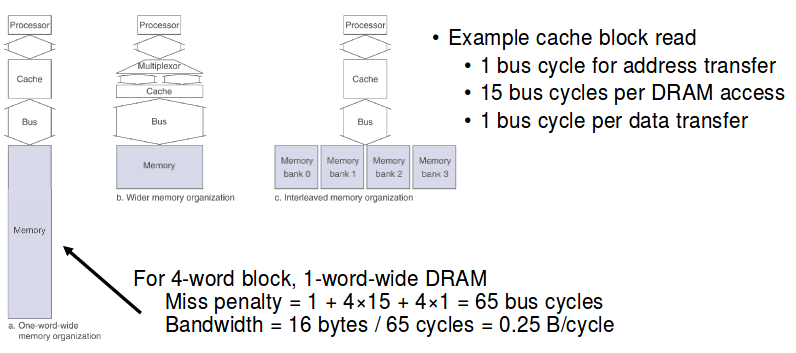
\includegraphics[scale=0.4]{lacache1.png}\\
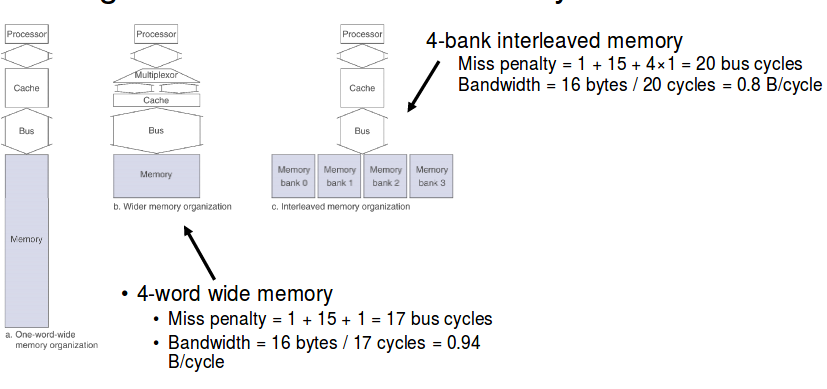
\includegraphics[scale=0.4]{lacache2.png}
\end{frame}
%------------------------------------------------------------------

\begin{frame} 
\Huge{\centerline{The End}}
\end{frame}

\end{document}